\chapter{Исследовательская часть}

\section{Технические характеристики}
Технические характеристики устройства, на котором выполнялись замеры по времени, представлены далее.
\begin{itemize}
	\item Процессор: AMD Ryzen 5 5500U\,--\,2.10 ГГц;
	\item Оперативная память: 16 ГБайт;
	\item Операционная система: Windows 10 Pro 64-разрядная система версии 22H2.
\end{itemize}

При замерах времени ноутбук был включен в сеть электропитания и был нагружен только системными приложениями.

\section{Демонстрация работы программы}
На рисунке \ref{img:demonstration} представлена демонстрация работы разработанного пргограммного обеспечение.  
\begin{figure}[h]
	\centering
	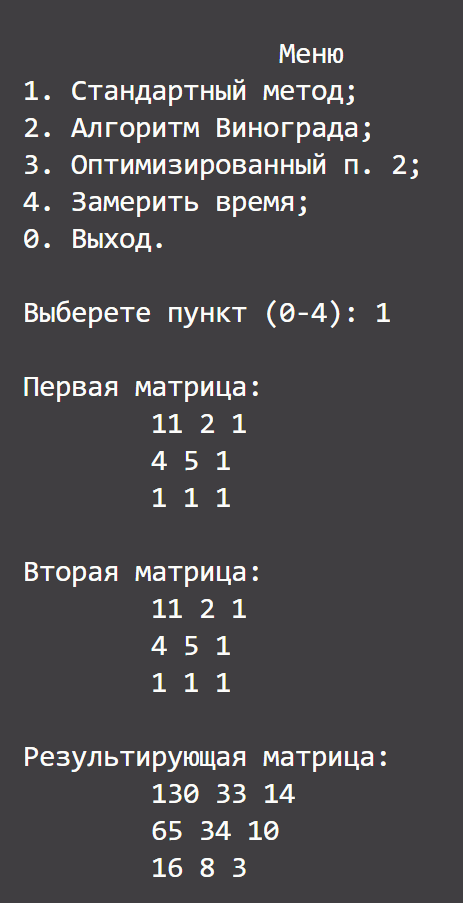
\includegraphics[height=0.3\textheight]{img/prog_work.png}
	\caption{Демонстрация работы программы}
	\label{img:demonstration}
\end{figure}

\section{Затраты по времени выполнения реализаций алгоритмов}
Все замеры проводились на квадратных матрицах. Поскольку замеры по времени имеют некоторую погрешность, замеры производились 100 раз, а затем вычислялось среднее арифметическое значение.

Результаты замеров приведены в таблицах \ref{tbl:time_even}--\ref{tbl:time_odd}.

На рисунках \ref{plt:time_01}--\ref{plt:time_03} приведены графики зависимостей работы алгоритмов от размеров матриц.

\begin{table}[h!]
    \caption{Результаты замеров времени (четные размеры матрицы)}
    \label{tbl:time_even}
	\centering
		\begin{tabular}{||c|c|c|c||}
			\hline
			& \multicolumn{3}{c|}{Время, мкс} \\ \cline{2-4}
			Размер матрицы & Стандартный & Виноград & (опт.) Виноград
			\csvreader{tables/time_even.csv}{}
			{\\\hline \csvcoli & \csvcolii & \csvcoliii & \csvcoliv} 
			\\
			\hline
		\end{tabular}
\end{table}

\begin{table}[h!]
    \caption{Результаты замеров времени (нечетные размеры матрицы)}
    \label{tbl:time_odd}
	\centering
		\begin{tabular}{||c|c|c|c||}
			\hline
			& \multicolumn{3}{c|}{Время, мкс} \\ \cline{2-4}
			Размер матрицы & Стандартный & Виноград & (опт.) Виноград
			\csvreader{tables/time_odd.csv}{}
			{\\\hline \csvcoli & \csvcolii & \csvcoliii & \csvcoliv} 
			\\
			\hline
		\end{tabular}
\end{table}

\begin{table}[h!]
    \caption{Результаты замеров времени (размер матрицы~--- степень двойки)}
    \label{tbl:time_ext}
	\centering
		\begin{tabular}{||c|c|c|c|c||}
			\hline
			& \multicolumn{4}{c|}{Время, мкс} \\ \cline{2-5}
			Размер матрицы & Стандартный & Виноград & (опт.) Виноград & Штрассен
			\csvreader{tables/time_ext.csv}{}
			{\\\hline \csvcoli & \csvcolii & \csvcoliii & \csvcoliv & \csvcolv} 
			\\
			\hline
		\end{tabular}
\end{table}

\clearpage

\begin{figure}[H]
	\centering
	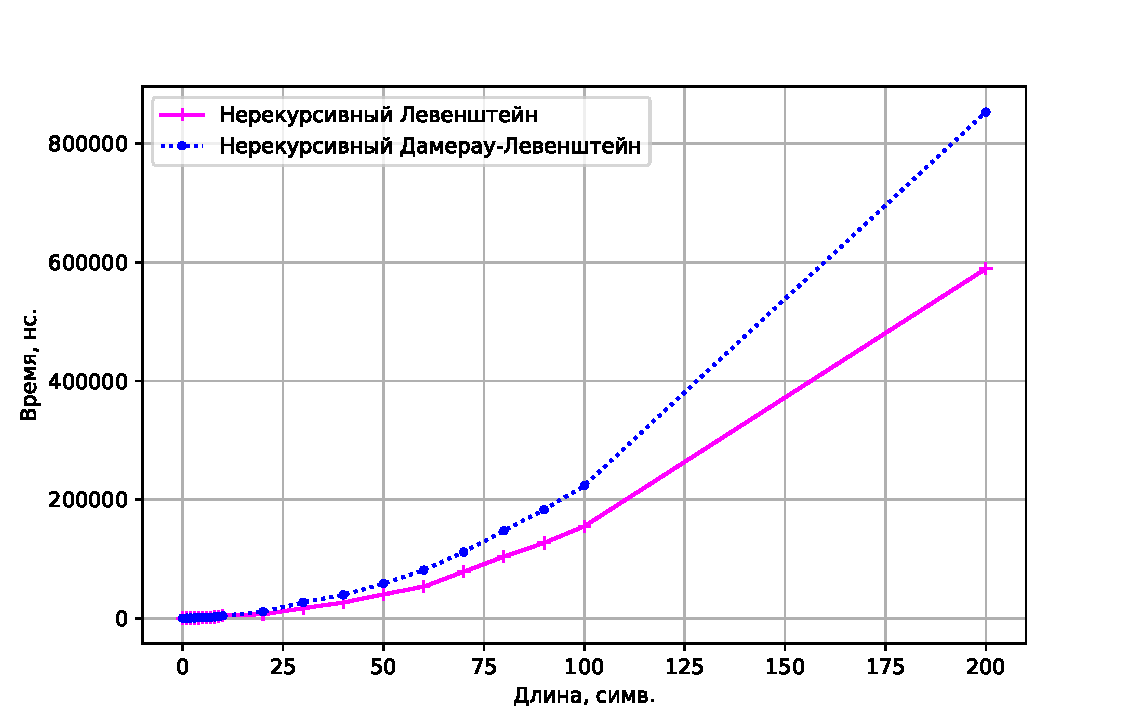
\includegraphics[height=0.4\textheight, page=1]{img/figures.pdf}
	\caption{Сравнение по времени алгоритмов умножения матриц на четных размерах матрицы}
	\label{plt:time_01}
\end{figure}

% \clearpage

\begin{figure}[H]
	\centering
	\includegraphics[height=0.4\textheight, page=2]{img/figures.pdf}
	\caption{Сравнение по времени алгоритмов умножения матриц на нечетных размерах матрицы}
	\label{plt:time_02}
\end{figure}

\clearpage

\begin{figure}[H]
	\centering
	\includegraphics[height=0.4\textheight, page=3]{img/figures.pdf}
	\caption{Сравнение по времени алгоритмов умножения матриц на размерах, равных степени двойки}
	\label{plt:time_03}
\end{figure}

\section{Затраты по памяти реализаций алгоритмов}
Введем следующие обозначения:
\begin{itemize}
	\item $size()$~--- функция вычисляющая размер в байтах;
	\item $int$~--- целочисленный тип.
\end{itemize}

Приведем теоретический расчет затрат по памяти для умножения двух матриц $A$ и $B$ размером $n \times n$, элементы которых типа $int$.

\subsection*{Стандартный алгоритм}
Затраты по памяти для реализации стандартного алгоритма приведены в формуле \ref{eq:mem_std}:
\begin{equation}
	\label{eq:mem_std}
	\begin{gathered}
		M_{std} = 3 \cdot size(int) + 3 \cdot size(int) + n \cdot n \cdot size(int) = \\ = (n^{2} + 6) \cdot size(int),
	\end{gathered}
\end{equation}
где, $3 \cdot size(int)$~--- переменные, хранящие размеры матриц;
\newline $3 \cdot size(int)$~--- переменные, используемые в циклах;
\newline $n \cdot n \cdot size(int)$~--- результирующая матрица.

\subsection*{Алгоритм Винограда}
Затраты по памяти для реализации алгоритма умножения методом Винограда приведены в формуле \ref{eq:mem_vin}:
\begin{equation}
	\label{eq:mem_vin}
	\begin{gathered}
		M_{vin} = M_{mulH} + M_{mulV} + M_{mul},
	\end{gathered}
\end{equation}
где $M_{mulH}, M_{mulV}$~--- память, используемая для хранения дополнительных массивов;
\newline $M_{mul}$~--- память, используемая при самом умножении матриц;

Соответствующие затраты представлены в формулах \ref{eq:mem_vin_1}--\ref{eq:mem_vin_2}
\begin{equation}
	\label{eq:mem_vin_1}
	\begin{gathered}
		M_{mulH} = M_{mulV} = n \cdot size(int) + 2 * size(int);
	\end{gathered}
\end{equation}
\begin{equation}
	\label{eq:mem_vin_2}
	\begin{gathered}
		M_{mul} = n \cdot n \cdot size(int) + 3 \cdot size(n) +
			\begin{cases}
				0, & \text{чётная} \\
				2 \cdot size(int), & \text{иначе}.
			\end{cases}
	\end{gathered}
\end{equation}

Итоговые затраты по памяти для реализации алгоритма Винограда:
\begin{equation}
	\label{eq:mem_vin_res}
	\begin{gathered}
		M_{mul} = (n^{2} + 2 \cdot n + 7) \cdot size(int) +
			\begin{cases}
				0, & \text{чётная} \\
				2 \cdot size(int), & \text{иначе}.
			\end{cases}
	\end{gathered}
\end{equation}

\subsection*{Оптимизированнный алгоритм Винограда}
Затраты по памяти для оптимизированной реализации алгоритма умножения методом Винограда идентичны формуле \ref{eq:mem_vin}.
$M_{mulH}$ и $M_{mulV}$ для данной релизации также совпадают.

Отличия появляются в самом умножении матриц, поскольку в целях оптимизации необходимо было некоторые значения хранить в отдельных переменных.
\begin{equation}
	\label{eq:mem_vinopt}
	\begin{gathered}
		M_{mul} = n \cdot n \cdot size(int) + 4 \cdot size(n) + \\ + n \cdot n \cdot \frac{n}{2} * size(int) + n \cdot n * size(int)
			\begin{cases}
				0, & \text{чётная} \\
				2 \cdot size(int), & \text{иначе}.
			\end{cases}
	\end{gathered}
\end{equation}

Итоговые затраты по памяти для оптимизированной реализации алгоритма Винограда:
\begin{equation}
	\label{eq:mem_vinopt_res}
	\begin{gathered}
		M_{mul} = (\frac{n^{3}}{2} + 2 \cdot n^{2} + 6 \cdot n + 4) \cdot size(int) +
		\begin{cases}
			0, & \text{чётная} \\
			2 \cdot size(int), & \text{иначе}.
		\end{cases}
	\end{gathered}
\end{equation}

\subsection*{Алгоритм Штрассена}
Рассчитаем затраты по памяти для каждого рекурсивного вызова.
\begin{equation}
	\label{eq:mem_stras}
	\begin{gathered}
		M_{mul} = (4 \cdot \frac{n}{2} \cdot \frac{n}{2} + 4 \cdot \frac{n}{2} \cdot \frac{n}{2} + \\ + 21 \cdot \frac{n}{2} \cdot \frac{n}{2} + n \cdot n) \cdot size(int),
	\end{gathered}
\end{equation}
где $4 \cdot \frac{n}{2} \cdot \frac{n}{2}$~--- 4 матрицы, на которые мы разбиваем нашу исходную матрицу;
\newline $13 \cdot \frac{n}{2} \cdot \frac{n}{2}$~--- временные матрицы, получаемые в ходе вычислений;
\newline $n \cdot n$~--- результирующая матрица.

Итоговые затраты по памяти для реализации алгоритма Штрассена:
\begin{equation}
	\label{eq:mem_stras_res}
	\begin{gathered}
		M_{mul} = \frac{33}{4} \cdot n^{2} \cdot size(int).
	\end{gathered}
\end{equation}

\section*{Вывод}
Исходя из данных, полученных в таблицах \ref{tbl:time_even}--\ref{tbl:time_ext}, можно сделать вывод, что лучше всего работает отмизированный алгоритм Винограда.
Стандартный же алгоритм умножения матриц работает медленнее по сравнению с двумя реалазиями алгоритма Винограда.
Модификации, используемые в оптимизированной реализации алгоритма также повлияли на его скорость работы. 
Также алгоритм Винограда при четном размере матрицы работает быстрее~--- это обусловлено проведением дополнительных вычислений для крайних строк и cтолбцов при нечетном размере. 
Таким образом, алгоритм Винограда стоит использовать при работе именно с матрицами, размер которых~--- четный.

Также на рис. \ref{plt:time_03} видно, что реализация алгоритма Штрассена выполняется намного дольше реализаций остальных алгоритмов, так как он требует дополнительных операций сложения и вычитаний матриц.

Из теоретических расчетов для потребляемой памяти, можно сделать вывод о том, что стандартное умножение требует наименьшее количество памяти. 
Наибольшие же затраты требует реализация алгоритма Штрассена, так как при каждом рекурсивном вызове необходимо разбивать исходные матрицы на 4 подматрицы, а также производить дополнительные опериции сложения и умножения.
Оптимизированная реализация алгоритма также требует больше памяти, по сравнению с неоптимизированной, так как используются дополнительные переменные для хранения некоторых предварительных вычислений.